% ===================== RESULTADOS =====================
\section{Resultados}
\label{sec:resultados}

Este capítulo presenta de forma cuantitativa y consolidada los resultados obtenidos mediante el modelamiento hidráulico numérico para las dos condiciones físicas de trazado evaluadas (superficial y enterrada mediante PHD) para los circuitos de salmuera y condensado.

% ─────────────────────────────────────────────────────────────────────────────
\subsection{Resultados del Modelamiento Hidráulico Dinámico}
\label{ssec:res_hidraulico}

La simulación se realizó considerando un caudal volumétrico de \SI{300.00}{\cubic\meter\per\hour} para cada línea en tuberías de \SI{12}{in} NPS: SDR 11 (ID = \SI{257.73}{\mm}) para salmuera saturada y SDR 13.6 (ID = \SI{268.68}{\mm}) para condensado. Los resultados de velocidad, número de Reynolds, pérdida de carga (cabeza hidráulica) y pérdida de presión dinámica se consolidan en la Tabla~\ref{tab:resumen_resultados}.

\begin{table}[htbp]
    \centering
    \caption{Resultados consolidados de la simulación hidráulica dinámica.}
    \label{tab:resumen_resultados}
    \small
    \setcounter{itemcount}{0}
    \begin{tabularx}{\textwidth}{@{}N>{\raggedright\arraybackslash}X>{\centering\arraybackslash}Xcccc>{\raggedright\arraybackslash}X@{}}
        \toprule
        \multicolumn{1}{c}{\textbf{Item}} & \textbf{Caso / Fluido} & \textbf{Config.} & \textbf{Q} & \textbf{Velocidad} & \textbf{Re} & \textbf{Cabeza $h_L$} & \textbf{Pérdida $\Delta P$} \\
        & & & \textbf{[m³/h]} & \textbf{[m/s]} & \textbf{[---]} & \textbf{[m]} & \textbf{[kPa]} \\
        \midrule
        & Salmuera saturada & Superficial & 300.00 & 1.60 & \num{3.09e5} & 3.277 & 38.56 \\
        & Salmuera saturada & Enterrada (PHD) & 300.00 & 1.60 & \num{3.09e5} & 3.332 & 39.21 \\
        & Condensado (agua) & Superficial & 300.00 & 1.47 & \num{3.90e5} & 2.546 & 24.97 \\
        & Condensado (agua) & Enterrada (PHD) & 300.00 & 1.47 & \num{3.90e5} & 2.592 & 25.42 \\
        \bottomrule
    \end{tabularx}
\end{table}

% ─────────────────────────────────────────────────────────────────────────────
\subsection{Carga de Presión Estática Global y Local Comparativa}
\label{ssec:res_estatico}

El trazado de la Perforación Horizontal Dirigida (PHD) desciende hasta una cota clave mínima de \SI{2542.75}{m.s.n.m.} en el tramo horizontal de fondo (Km 16.5). En una condición estática de parada con libre comunicación (comportamiento global), la presión estática en el cruce está gobernada por la cota del tanque de quiebre atmosférico de salmuera ($2658.24\ \text{m.s.n.m.}$) y, para el condensado, por la estación de bombeo ($2597.00\ \text{m.s.n.m.}$, valor provisional). Si se implementan válvulas de aislamiento intermedias en los puntos de conexión, la presión estática se limita al desnivel local del sifón. La Tabla~\ref{tab:resultados_estatico} presenta el análisis comparativo de la presión estática hidrostática entre el tramo superficial original y el enterrado (PHD) para ambos escenarios de operación.

\begin{table}[htbp]
    \centering
    \caption{Presiones hidrostáticas estáticas comparativas en el tramo Km 16.5.}
    \label{tab:resultados_estatico}
    \small
    \setcounter{itemcount}{0}
    \begin{tabularx}{\textwidth}{@{}N>{\raggedright\arraybackslash}X>{\centering\arraybackslash}Xccc@{}}
        \toprule
        \multicolumn{1}{c}{\textbf{Item}} & \textbf{Fluido / Servicio} & \textbf{Config.} & \textbf{Cabeza estática $dH$} & \textbf{Presión estática} & \textbf{Presión estática} \\
        & & & \textbf{[m]} & \textbf{[kPa]} & \textbf{[bar]} \\
        \midrule
        \multicolumn{6}{l}{\textit{Escenario A: sin válvulas de aislamiento (comportamiento global)}} \\
        & Salmuera saturada & Superficial (original) & 99.89 & \num{1175.62} & 11.76 \\
        & Salmuera saturada & Enterrada (PHD) & 115.49 & \num{1358.96} & 13.59 \\
        & Condensado (agua) & Superficial (original) & 38.65 & \num{379.18} & 3.79 \\
        & Condensado (agua) & Enterrada (PHD) & 54.25 & \num{532.16} & 5.32 \\
        \midrule
        \multicolumn{6}{l}{\textit{Escenario B: con válvulas de aislamiento (comportamiento local)}} \\
        & Salmuera saturada & Superficial (original) & 0.00 & 0.00 & 0.00 \\
        & Salmuera saturada & Enterrada (PHD) & 15.60 & 183.58 & 1.84 \\
        & Condensado (agua) & Superficial (original) & 0.00 & 0.00 & 0.00 \\
        & Condensado (agua) & Enterrada (PHD) & 15.60 & 152.98 & 1.53 \\
        \bottomrule
    \end{tabularx}
\end{table}

La Figura~\ref{fig:perfil_esquematico} presenta el perfil longitudinal esquemático del cruce por PHD en el Km~16.5, con las cotas de referencia (tanque de quiebre, terreno local y fondo del sifón) y las presiones estáticas de salmuera correspondientes a los escenarios global y local aislado.

\newpage
\begin{figure}[H]
    \centering
    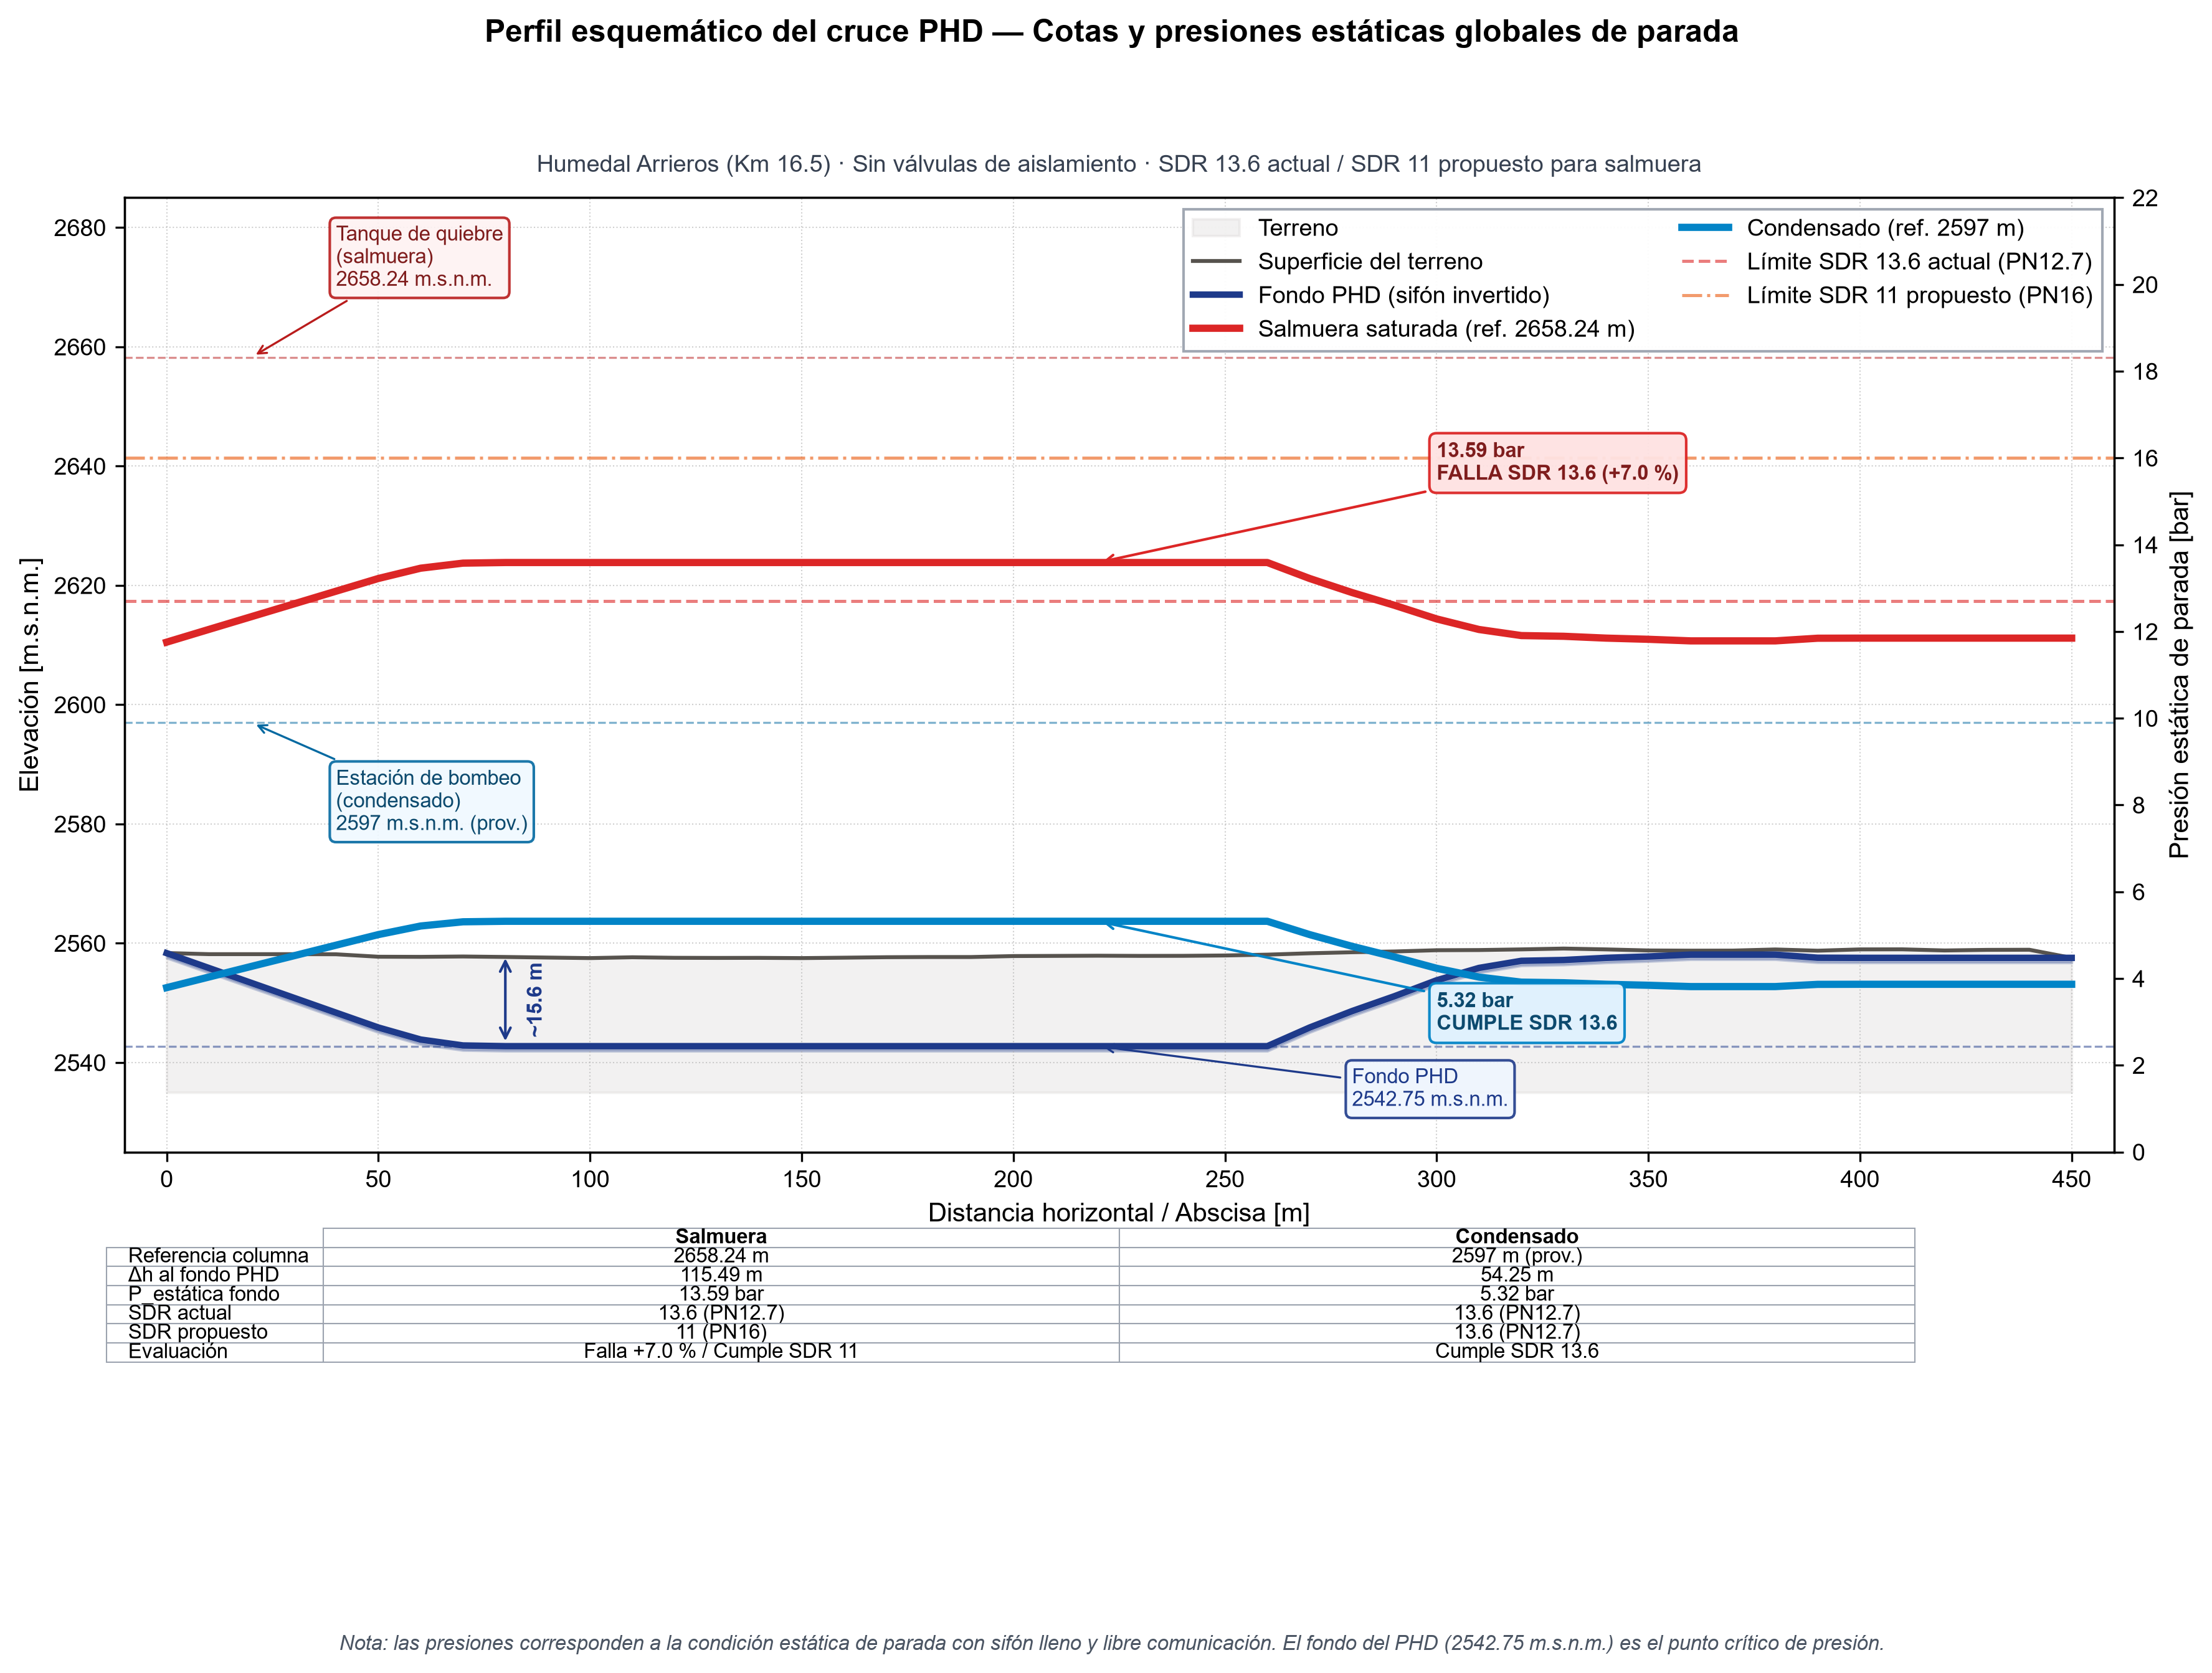
\includegraphics[width=\textwidth,height=\textheight,keepaspectratio]{assets/perfil_esquematico.png}
    \caption{Perfil esquemático longitudinal del cruce PHD en el Km 16.5 (Humedal Arrieros) con cotas de referencia y presiones estáticas de salmuera saturada.}
    \label{fig:perfil_esquematico}
\end{figure}

La reducción de la presión estática de salmuera de \SI{18.90}{bar} a \SI{13.59}{bar} se debe a que la columna hidrostática real no parte de la Mina de Sesquilé, sino del tanque de quiebre atmosférico ubicado a 2660 msnm (mina 2704 msnm). Esta presión excede la capacidad de la tubería actual SDR~13.6 (PN12.7) en un \SI{7.0}{\percent}, por lo que la línea de salmuera se rediseña a SDR~11 (PN16), la cual cumple con un margen del \SI{15.1}{\percent}. El condensado se mantiene en SDR~13.6 porque su presión estática global de \SI{5.32}{bar} cumple ampliamente.

